\chapter{外文资料翻译}
\label{cha:engorg}

\title{供电网格分析中的多重网格技术}

\textbf{摘要}:
现代的超大规模集成电路设计里面包括规模巨大的供电网络,供电网络需要用越来越低的电压分配大量的供电源。网格中的电压降减少了噪声区间的范围,增加了门延迟,造成了一系列的
性能影响。用传统的电路模拟方法对供电电压的完整性进行检验是一个不现实的方法,因为时间与内存开销过大。我们提出了一个新的基于多重网格的供电网络分析技术。原供电网格
被缩小到一个更粗的网格结构,然后这个网格的解会被映射回原来的细网格中。实验结果证明了我们提出的方法效率非常高,适合供电网格的直流分析与瞬态分析。

\section{引言}

近年来,对高性能与低能耗的VLSI设计的需求越来越高。高性能的实现主要通过技术扩大,功能增强以及更好的设计。另一方面,一个常用的低能耗的设计方法是减少供电电压,因为
芯片功率$P$是与供电电压$V_{DD}$的平方成正比的。所以,对于高性能与低能耗的需求导致了现代的VLSI设计以少量的特点大小、增强的功能、低供电电压为特点。

增强的芯片功能导致了对巨大功率分布网络的需求,这也被成为供电网格因为他们经常是一个网格状的拓扑结构。更低的供电电压,另一方面,使得电压在供电网格范围内的抖动会带来
很大的影响,进一步会导致电路的故障。电压值的降低会使得逻辑门与晶体管元件的实际供电电压比理论值要小。这会导致更窄的噪声区间,更高的逻辑门延迟,以及整个电路的降速。
噪声区间变窄会导致电路里特定逻辑门的错误的开关切换。更高的逻辑门延迟在另一方面也会降低电路的速度导致时序要求无法满足。所以,一旦电压的降低超过了一定的设计阈值,
电路的正常运行就没法保证了~\cite{dharchoudhury1998design, yim1999floorplan, steele1998full}。

因此,很显然在现代的VLSI设计中,供电网格正在成为制约性能的一个重要因子。所以对供电网格的高效分析~\cite{nassif2000fast, zhao2002hierarchical}是很有必要的;
一能预测性能,二能改善性能。因为供电网格的规模大的特性,现在的分析方法都不能满足需求。所以,一个时间与内存效率都高的分析技术显得格外重要。

\section{供电网格的建模与分析}

在这一节中,我们会讨论供电网格的基本模型与分析技术。具体来说,\ref{}节会讨论如何对传统的供电网格、电流源、二极管进行建模,以适应高效精确的分析。另一方面\ref{}节会
介绍基本的分析技术并讨论一些提升分析速度的技术细节。

\subsection{供电网格的建模}


从供电网格到外部供能电源($V_{DD}$)的连接被称为电力来源,因为电流是通过这个连接从外部电源流入网格的。电源漏极,另一方面,指的是那些从供电网格中获取电流的元件。比如说,
晶体管、逻辑门、触发器、时钟缓存器、内存单元、寄存器阵列、IO缓存区等都被认为是电源漏极。

供电网格分析的第一步包括对电网以及电源和漏极进行建模~\ref{chen1998interconnect}。 网格,电力来源和漏极的建模涉及准确性和速度之间的权衡。 模型越复杂分析结果越准确,
解决方案越昂贵(在内存和CPU时间方面)。

\begin{figure}[H] % use float package if you want it here
  \centering
  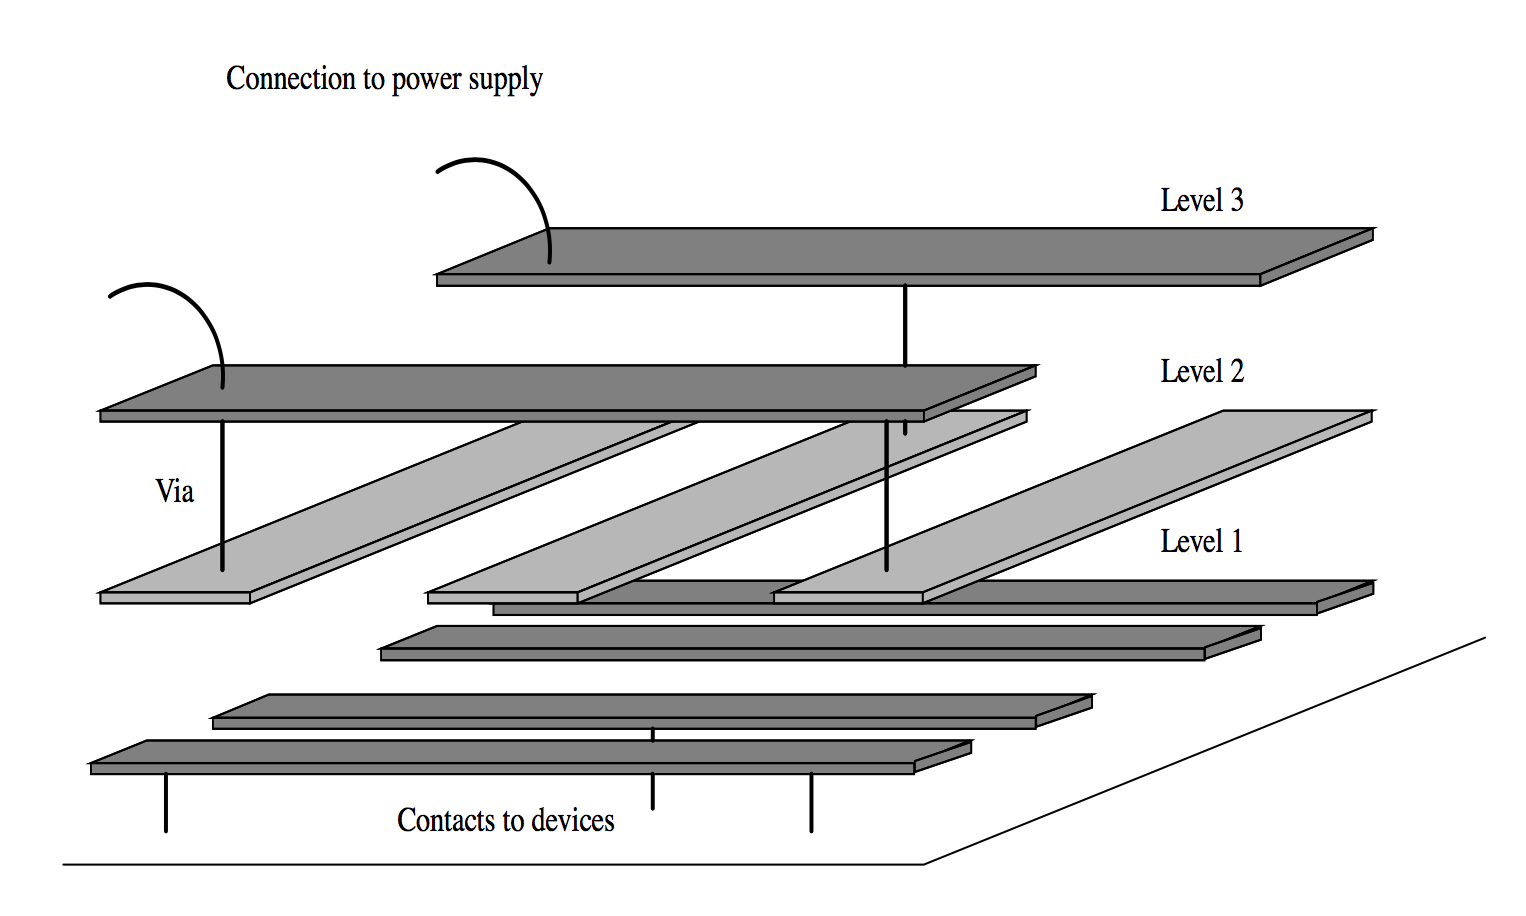
\includegraphics[height=8cm]{a1}
  \caption{供电网络的组成}
  \label{fig:a1}
\end{figure}

通常,如图\ref{fig:a1}所示,集成电路内的功率分配由顶层金属层完成,顶层金属层通过层间通孔向下连接,最后到达目标器件。我们遵循如\cite{chen1998interconnect}所述的建模方法,其中金属线和通孔被建模为由电阻性,电容性和非电感性元件组成的线性、时不变的网络。 对于诸如微处理器的现代集成电路,这样的网络可以轻易地包括数百万个节点和数千万个元件。

至于电源和漏极,其型号可能相当复杂。 电源的型号包括复杂的封装和电路板型号。 另一方面,电源漏极的模型可以解释供电网格,底层非线性电路与跨芯片传播的时变信号之间的复杂相互作用。 然而,供电网格巨大的规模使得电源和漏极系统中只能使用最简单的模型。 因此,电力来源被建模为简单的恒定电压源,功率消耗被建模为独立的时变电流源。

鉴于上述情况,完整的供电网格模型由一个由恒定电压源和时变电流源激励的RLC元件组成的线性网络。 需要注意的是,没有任何网络的RLC元件是连接到地的,所有的电压源都在某些网格节点和地之间,并且所有的电流源(漏极)都在网格节点和地之间。 这种系统的行为可以通过修改的节点分析(MNA)~\cite{pillage1998electronic}公式来表达:
\begin{align}
Gx+C\dot{x}=u(t)
\label{eq:eq1}
\end{align}
其中$x$是节点电压、电源、电导电流的向量;G是电导矩阵;C包括电容和电感项,$u(t)$包括电力来源和漏极的贡献。 事实上,$u(t)$具有三种行:i) 具有正$V_{DD}$值的行,其对应于连接到电源的节点,ii) 具有负电流值(或电流总和)的行,其对应于连接到一个或多于一个功率消耗的节点,以及iii) 具有0的行,其对应于所有其他节点。

接下来,我们忽略片上电感的影响,并假设电网仅被建模为RC网络。 这是由于在当今的技术中,电网中的片上电感太小而不能显著影响分析结果。 总而言之,电网被建模为RC网络,电源被建模为恒定电压源,功率消耗被建模为时变电流源。

\begin{figure}[H] % use float package if you want it here
  \centering
  \includegraphics[height=6cm]{a2}
  \caption{3x3的供电网格例子}
  \label{fig:a2}
\end{figure}

\begin{figure}[H] % use float package if you want it here
  \centering
  \includegraphics[height=4cm]{a3}
  \caption{逆转器引去的电流}
  \label{fig:a3}
\end{figure}

图\ref{fig:a2}表示出了在节点1处具有一个电压源(由X指示)和节点5和7处的两个电流源(由点指示)的$3x3$电网。 该示例表示出在每层中具有三根电线,节点1处有一个电压源,有两个功率消耗(一个从节点5引去电流,另一个从节点7引去电流)的两层电网的模型。一个关联着逆转电源漏极的电流源的示例如图\ref{fig:a3}所示,以数学的形式表达如下(其中$t$是以纳秒为单位的时间,I是以毫安为单位的电流):

\begin{align}
I=\begin{cases}
    410^6t & 0\leq t \leq 0.2510^{-9}\\
    -410^6 + 210^{-3} & 0.2510^{-9} \leq t \leq 0.510^{-9}
\end{cases}
\end{align}

\subsection{供电网格的分析}

由于供电网格的大规模,一般电路仿真器如Spice~\cite{nagel1975spice2}不足以进行电网分析,因为CPU时间和内存有一定的限制。 标准模拟器的低效率是因为 (a)它们需要电路的元件都近似,该电路需要将常规的电路几何结构转换成一组扩展的等效电路元件,(b)它们使用通用的解决方法, 即使是难解的方程组也要保证正确性。 相比之下,供电网格在空间(非常规则)和时间(阻尼性的)方面表现良好。 这让我们想到了一种可以利用这些特性的供电网格专用模拟器。

求解式子\ref{eq:eq1}需要使用一些数值积分公式。 通常会选择逆向欧拉(BE)积分公式,主要是由于其稳定性的特点~\cite{pillage1998electronic}。对式子\ref{eq:eq1}应用后向欧拉得到一组线性方程:
\begin{align}
(G+C/h)x(t+h)=u(t+h)+x(t)C/h
\label{eq:eq2}
\end{align}
可以被简化成$A'x(t+h)=b'$,其中$A'=G+C/h$并且$b'=u(t+h)+x(t)C/h$。

式子\ref{eq:eq2}的解决方案要求矩阵$A'= G + C / h$的逆矩阵,其独立于x,时不变,规模大但是系数稀疏。 然而,我们注意到,如果我们将时间步长h保持恒定,那么只需要一个初始的矩阵分解,和每个时间步长的向前/向后的解。 因为对于大规模的矩阵,矩阵分解比前向/后向解决方案明显更花销更高~\cite{golub2012matrix},所以使用恒定的时间步长可以大大节省计算成本。 时间步长需要保持足够小以确保解决方案的准确性。 为了在数字电路的电网分析中的应用,我们发现每个时钟周期使用100个步长(即$h = 0.01 * T$)就足够了。

\begin{figure}[H] % use float package if you want it here
  \centering
  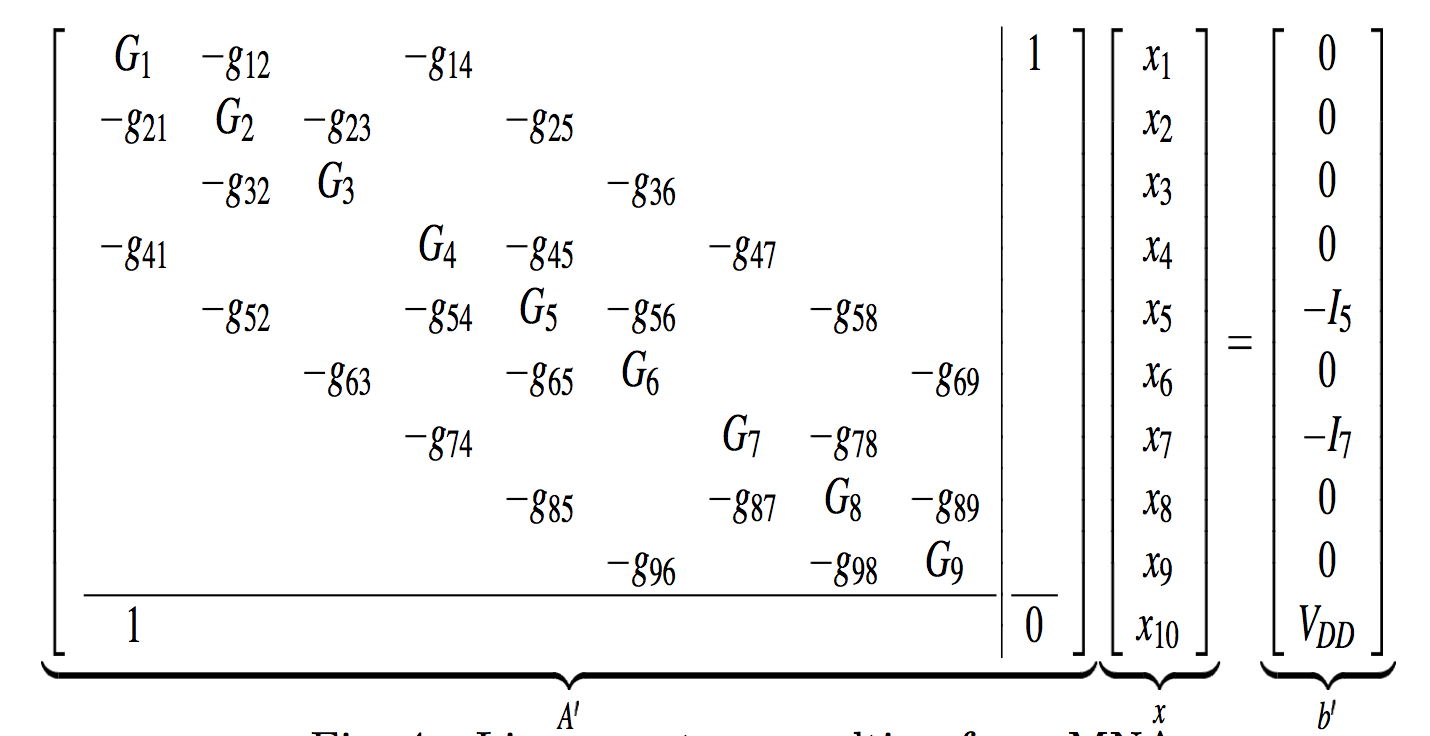
\includegraphics[height=4cm]{a4}
  \caption{根据修改的节点分析法得到的矩阵}
  \label{fig:a4}
\end{figure}

为了更好地解释供电网格的分析过程,将修改的节点分析法(MNA)应用于图\ref{fig:a2}给出的示例,从而得到了图\ref{fig:a4}所示的线性系统。

令$N$为电网的节点数。 然后,在图\ref{fig:a2}所示的示例网格中,$N = 9$,因为网格是3x3。此外,存在一个电压源,这意味着$A'$矩阵是10x10矩阵,其中前9个方程是应用KCL方程在所有9个节点上,最后一个方程是节点1处的电压源分配的KVL方程。 电流源方面,节点5和7中的电流源出现在右侧矢量$b'$中。 另一方面,$g_{ij}$定义了两个相邻节点$i$和$j$之间的电导。 因此,$g{ij} = g{ji}$导致$A'$矩阵是对称的。 此外,A矩阵的对角元素定义如下:
\begin{align}
    G_i = \sum_{j\in N_i} |g_{ij}| + C_i/h
\end{align}
其中,$C_i$是节点$i$的电容,$h$是时间步长,$N_i={j|g{ij}\neq 0}$是节点$i$的邻接点集合。

通常,线性系统$A'x = b'$的系统矩阵$A'$是对称的,但不一定是正定的~\cite{9}。然而,该问题可以被重新归纳到对称的正定矩阵$A$上。基本上,MNA公式通过在电源节点处运用KCL和KVL方程来构建线性系统$A'x = b'$,以及剩下的网格节点的KCL方程。然后,所得到的线性系统的解$x$给出了所有电网节点处的电压以及由不同电压源提供的电流。然而,如果我们只对所有电网节点的电压感兴趣,那么我们可以忽略与电源节点相对应的KCL方程。此外,电源节点处的电压已知为电源电压$V_{DD}$。因此,我们可以通过将电源的值替换为所有电源节点的电压,并忽略电源节点的KCL方程来简化问题。

\begin{figure}[H] % use float package if you want it here
  \centering
  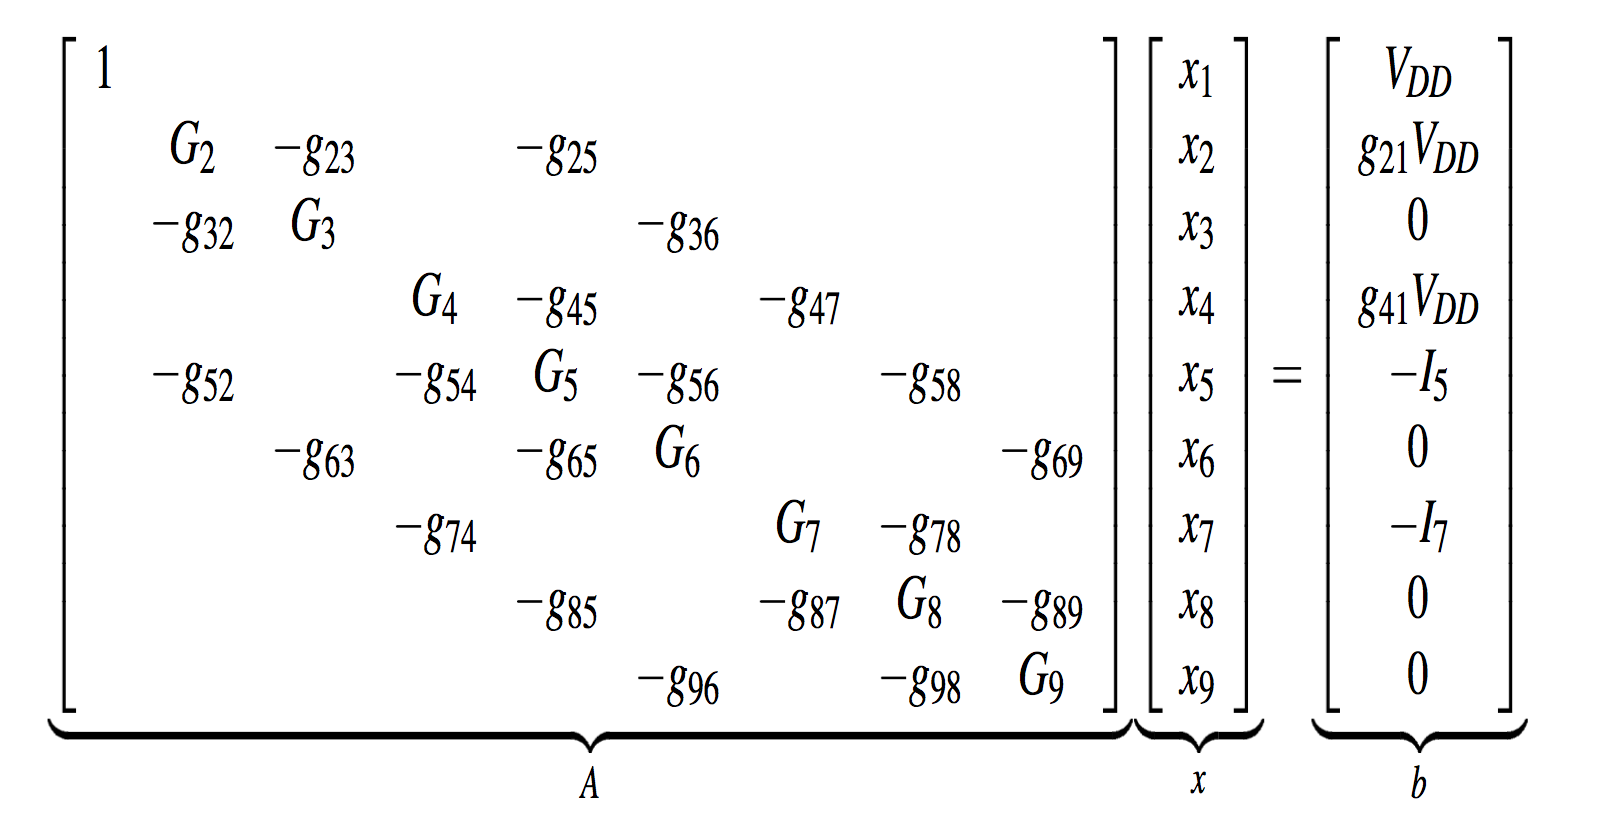
\includegraphics[height=4cm]{a5}
  \caption{变形后的线性方程系统}
  \label{fig:a5}
\end{figure}

我们通过将这种变形的方法应用于上述的3x3网格示例来说明。 节点1具有电压源,因此我们用节点1处的KVL方程代替节点1处的KCL方程。 所得到的系统如图\ref{fig:a5}所示。

观察到右侧也被改变了,产生了新的向量$b$。 很明显,得到的矩阵$A$仍然是对称的;进一步,也是对称正定的。 为此,先注意到$\forall i, |g_{ij}|=|g_{ji}|$。结合\ref{eq:eq3}中的结果,可以得到:
\begin{align}
|G_i| = \sum_{j\in N_i} |g_{ij}|+C_i/h=\sum_{j\neq i}|g_{ij}|+C_i/h\geq \sum_{j\neq i}g_{ij} \quad \forall i
\label{eq:eq4}
\end{align}
方程\ref{eq:eq4}适用于每个节点$i$,等效于系统矩阵$A$的每一行。这表明变形后的矩阵$A$是对角占优的,并且已经指出$A$也是对称的。 所以,$A$是一个对称和正定矩阵~\cite{golub2012matrix}。 事实上,$A$是M-矩阵~\cite{berman1994nonnegative},因为它满足以下条件:
\begin{enumerate}
\item $a_{ii}>0 \quad \forall i$
\item $a_{ij}\leq 0 \quad \forall i\neq j$
\item $a_{ii}\geq \sum_{j\neq i}|a_{ij}| \quad \forall i$
\item $a_{ii}>\sum_{j\neq i}|a_{ij}| \quad \exists i$
\end{enumerate}
其中$a_{ij}$矩阵$A$第$i$行第$j$列的元素。所以,在剩下的篇幅里,我们会利用$A$是一个非奇异的$M$矩阵的性质。

\section{多重网格方法}

在精心设计的供电网格中,电阻远远小于等效吸收电阻,因为电网需要为所有的漏极提供稳定的电压。 这将导致局部电力干扰,将被扩散到比引起干扰的区域大得多的区域上。 这种扩散导致空间平滑的电压分布,并且是的我们的对供电网格的解决方案可以利用这种平滑度来加速解决过程。

此外,我们注意到,电网分析会产生一个与二维抛物线偏微分方程(PDE)的有限元离散化相似的线性方程组。 这促使我们将电网问题视为连续PDE的离散化,其中需要在空间固定的点解出所需值。 因此,解决PDE的有效方法值得考虑作为电网问题的潜在解决方案。

近年来,多重网格方法(MG)已经成为解决平滑PDE的标准解法~\cite{briggs2000multigrid,brandt1973multi,hackbusch2013multi}。 多重网格涉及两个基本操作:i)松弛操作和 ii)粗网格校正。松弛操作涉及运行迭代求解器的几次迭代,以平滑误差分量;也就是减少高频误差分量。 另一方面,粗网格校正涉及将问题映射到较粗的网格,在较粗的网格上解决问题,然后将解决方案映射回原始网格。 这两个相辅相成的步骤一起提供了一种解决PDE的有效技术。 因此,在本文中,我们认为可以把它用于电网分析中。

虽然经典的迭代方法由于网格维度增加(等效的网格间距减小)而收敛速度大大降低时,但是多网格性能并不能确定。 事实上,已经证明多网格具有最佳的性能,因为可以用O$(n)$复杂度来解决$n$个方程的系统。多重电网技术 不仅是最优复杂度的,而且所涉及的常数都足够小,让多重电网优于其他方法~\cite{hackbusch2013multi}。 我们应该在这里指出,多重网格方法属于像Jacobi和Gauss-Seidel这样的迭代求解器类别,而不是像高斯消除那样的直接求解器。

我们已经提到,经典迭代方法的分析与对多重网格很有关系。 所以我们将从对经典迭代方法的简要分析开始。 给定线性系统$Ax = b$和初始猜测$x_0$,迭代方案涉及如下:
\begin{align}
\hat{x}^{k+1}=\hat{x}^{k}+M^{-1}(b-A\hat{x}^k)
\end{align}
其中$k$是迭代的当前次数,$\hat{x}^k$是第$k$轮迭代后的对解的估计值。对于$M$,它是一个易于求解的矩阵,使得$M^{-1}\approx A^{-1}$。

令$e = x-\hat{x}$为精确解$x$与近似解$\hat{x}$之间的差。 可以看出,误差可以表示为低频和高频傅里叶模式的线性组合~\cite{briggs2000multigrid}。 此外,经典迭代法的分析导致以下观察~\cite{briggs2000multigrid, stuben1982multigrid}:
经典迭代方法有效地降低了高频误差分量,但在降低低频误差分量方面效率不高。

为了避免经典方法的局限性,多重网格方法由两个互补的部分组成:1) 松弛操作,可以减少高频误差;2)粗网格修正,可以减少低频误差。

\begin{figure}[H] % use float package if you want it here
  \centering
  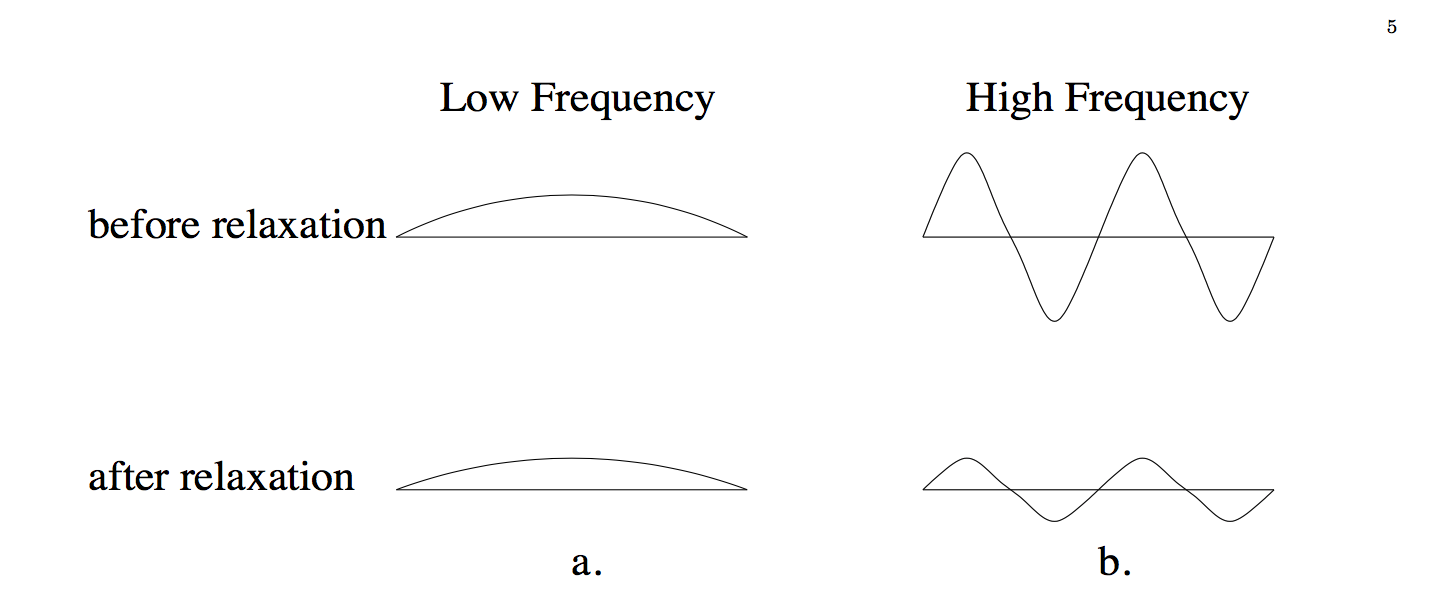
\includegraphics[height=7cm]{a6}
  \caption{迭代方法的松弛效果}
  \label{fig:a6}
\end{figure}

松弛操作涉及到经典迭代求解器的几次迭代。从观察结果可以看出,经典的迭代方法是良好的平滑器,如图\ref{fig:a6}所示~\cite{stuben1982multigrid}。另一方面,粗网格校正将问题映射到较粗的网格,解决映射问题,并将得到的解映射回到精细的网格。两个网格(细和粗)之间通信所需的关键工具是网格间转移子,分别是网格限制子和网格延长子。粗网格校正的一个直观的动机是粗网格的解决方案通常为细网格上的迭代求解器提供了良好的初始猜测,从而能加速收敛。这种方法的另一个动机是,如图\ref{fig:a7}所示,细电网$\Omega^h$的低频误差分量在粗网格$\Omega^{2h}$出现更多的振荡。所以应在较粗的网格上进行松弛操作,减少这些误差成分。

\begin{figure}[H] % use float package if you want it here
  \centering
  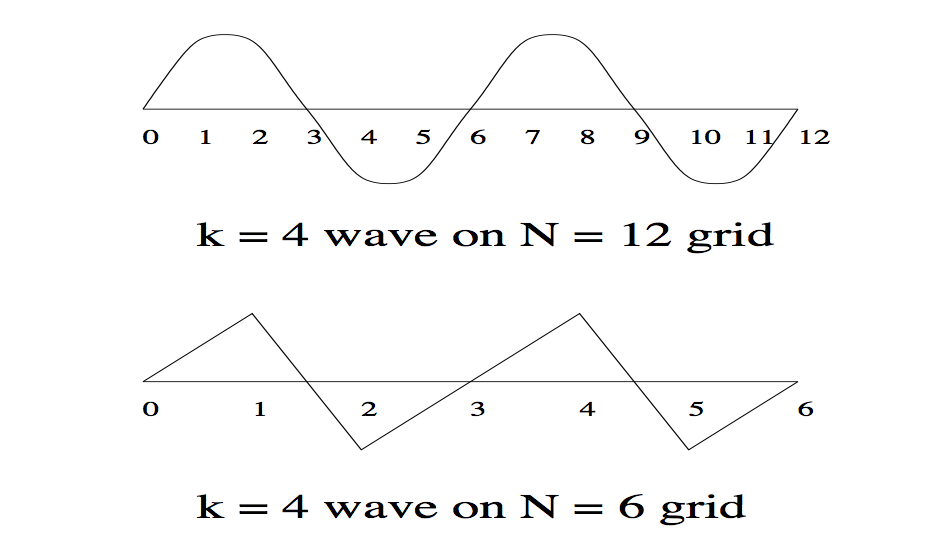
\includegraphics[height=6cm]{a7}
  \caption{迭代方法的松弛效果}
  \label{fig:a7}
\end{figure}

多重网格技术的工作如下~\cite{briggs2000multigrid}。 从精细网格开始,进行几个松弛步骤应用以减少误差中的高频部分。 然后误差中的低频部分通过粗网格校正也得到了降低。 这产生了下面的这个高效率的算法,我们称之为V-循环多重网格方法。 在下文中,$R_h^{2h}$和$P^h_{2h}$分别对应于限制操作子和延长操作子。 另一方面,$V^h$表示V-cycle算法;并且用$h$定义V-cycle算法被调用的深度。 $v_1$和$v_2$是要执行的迭代次数,是常数。 这些常数是依据经验选择的,通常是2或3。

\begin{align*}
\hat{x}^h \leftarrow V_h(\hat{x}^h, b^h)
\end{align*}
\begin{enumerate}
\item 用初始解$\hat{x}^h$对$A^hx^h=b^h$进行$v_1$次迭代松弛操作;
\item 如果目前的$\Omega^h$是可以容许的最粗的网格,那么去第四步;否则令$b^{2h}\leftarrow R_{h}^{2h}(b^h-A^h\hat{x}^h)$,$\hat{x}^{2h}\leftarrow 0$,$\hat{x}^{2h}\leftarrow V^{2h}(\hat{x}^{2h}, b^{2h})$;
\item 修正:$\hat{x}^{h} \leftarrow \hat{x}^h + P^h_{2h}\hat{x}^{2h}$
\item 用初始解$\hat{x}^h$对$A^hx^h=b^h$进行$v_2$次迭代松弛操作;
\end{enumerate}


\section{供电网格中的多重网格分析方法}

在这一节中,我们讲讲述这个供电网格分析的新方法的各种细节。这个技术使用了多重网格理论的一般思想。然而,它独特地瞄准着供电网格问题的细则,从而产生了一个更高效的算法。

供电网格分析包含三步:1)对供电网格、电流源、漏极进行建模;2)使用改进的节点分析法(MNA)对线性系统$Ax=b$进行形式化;3)对$Ax=b$进行求解,从而得出供电网格所有节点的电压降。

前面已经讨论了对供电网格,电流源和漏极进行有效分析时模型建立的必要性。 此外,通过应用改进的节点分析(MNA),线性系统$Ax = b$的公式已经在前面已经说明过了。 因此,仍然要讨论的是如何有效地解决所得到的线性系统$Ax = b$。

如第三节所述,电网问题最初是一个离散的问题,因此启发我们使用代数多重网格的算法。 然而,成功应用代数多网格需要定义一个良好的插值算子。 这规定了一个满足以下要求的网格缩减(粗化)机制:

\emph{对于每个被删除的节点$i$,所有强连接到$i$的节点$j$要么被继续保留,要么强制连接到至少一个节点$k$,其中$k$被保留并且强连接到$i$。}

满足上述要求可能导致网格缩减的效率低下。 具体来说,所得到的粗化的网格可能不够粗糙;也就是说,网格缩减只能移除少量的节点。 这就意味着算法效率不高,在CPU时间和内存方面花销很高。 因此,为了避免算数多重网格的限制,我们提出了一种类似于使用标准多重网格的网格缩减算法的算法。 然而,由于典型的供电网格可能是不规则的,我们的算法被设计为能有效地处理供电网格的不规则性,并且在每次迭代时产生显着减小的较粗网格。

一旦网格被缩减,我们提出的方法定义了插值算子,以满足代数多重网格方法的要求。 也就是说,插值算子被定义为使得不能很好地减少的误差分量位于其范围空间中的算子。假设插值运算符满足:
\begin{align}
e^h_i=e^H_i \quad \text{if }i\text{ is kept and} \\
e^h_i=\sum_{j\in N_i} \frac{|a_{ij}|}{a_{ii}} e^H_j \quad \text{if }i\text{ is removed}
\end{align}
其中$h$和$H$分别表示细网格与粗网格。

这个定义可以保证误差在于插值算子所定义的范围空间内,因为$e_h = P_H^he^H$。 注意如果$|a_{ij}|/a_{ii}$很小,那么节点$j$的效果可以忽略不计。 也就是说,将已删除的节点$i$的电压与强连接到$i$的那些节点进行插值是足够的。 基于此,我们从去除的节点$m$与$m$强连接的节点的电压进行插值。 由于网格的几何形状是已知的,因此可以容易地识别出与$m$强连接的且仍保留着的节点。 通常来说,这些将是$m$的几何邻居和/或其这些邻居对应的邻居。

因此,提出的方法结合了标准与代数这两种多重网格技术的优点,同时避免了它们的局限性。 此外,所提出的方法与常规多重网格相比还有另一个显着的优点。 如前所述,多重网格包含两个主要部分:松弛(或平滑)操作和粗网格校正。 松弛操作的作用基本上是平滑误差分量,而粗网格校正的作用是近似估计那些平滑的误差分量。 然而,在电网中,误差分量通常是平滑的,因为供电网格被设计成在网格上具有平滑的电压变化。 因此,在解决电网问题时,可以忽略多重网格的松弛步骤,仅集中在粗网格校正步骤上。 这正是我们提出的方法所做的,下面的实验结果表明,这种假设带来了显着的加速,同时只引入了非常小的误差。

假设平滑的电压变化,忽略松弛步骤,我们提出的方法属于直接求解器的类型,而不是基于迭代求解器的多重网格技术。 当进行瞬态分析时,这会导致算法获得进一步加速。 给定一个初始电网$\Omega^h$及与之相关的线性系统$A^hx^h = b^h$,提出的方法可以总结如下:
\begin{enumerate}
\item 在细网格上进行缩减算法,产生一个粗网格$\Omega^{2h}$;
\item 定义插值操作子$P_{2h}^h$;
\item 如果$\Omega^{2h}$不够粗,那么先把$\Omega^{2h}$拷贝到$\Omega^h$上,然后更新插值操作子$P_{2h}^h$,然后返回第一步进行递归;另一方面,如果$\Omega^{2h}$足够粗,那么把问题映射到粗网格上:$A^{2h}=(P_{2h}^h)^TA^hP^h_{2h}$ 并且
$b^{2h}=(P^h_{2h})^Tb^h$,然后在粗网格上求解$A^{2h}x^{2h}=b^{2h}$,最后把解映射回细网格中:$x^h=P^h_{2h}x^{2h}$。
\end{enumerate}

注意到,对网格的缩减标准是是用户自定义的。 网格粗略足够的标准涉及程序精度和运行速度之间的权衡。 供电网格越粗,解决方案越快,但精度越低。 通常,足够粗的网格指的是问题的大小足够小以至于能快速有效解决的网格。 在我们的实现中,四个级别的供电网格缩减(根据经验)足以产生可以有效解决的缩减系统。

在本节的剩下部分中,我们将关心粗网格校正过程,一旦选择了粗化策略并定义了插值算子,这一过程就被完全确定了。 我们定义和讨论了网格缩减算法。 然后我们将说明插值算子是如何定义的。 最后,讨论了使用多重网格技术进行瞬态分析的优点。

\subsection{网格缩减}

\begin{figure}[H] % use float package if you want it here
  \centering
  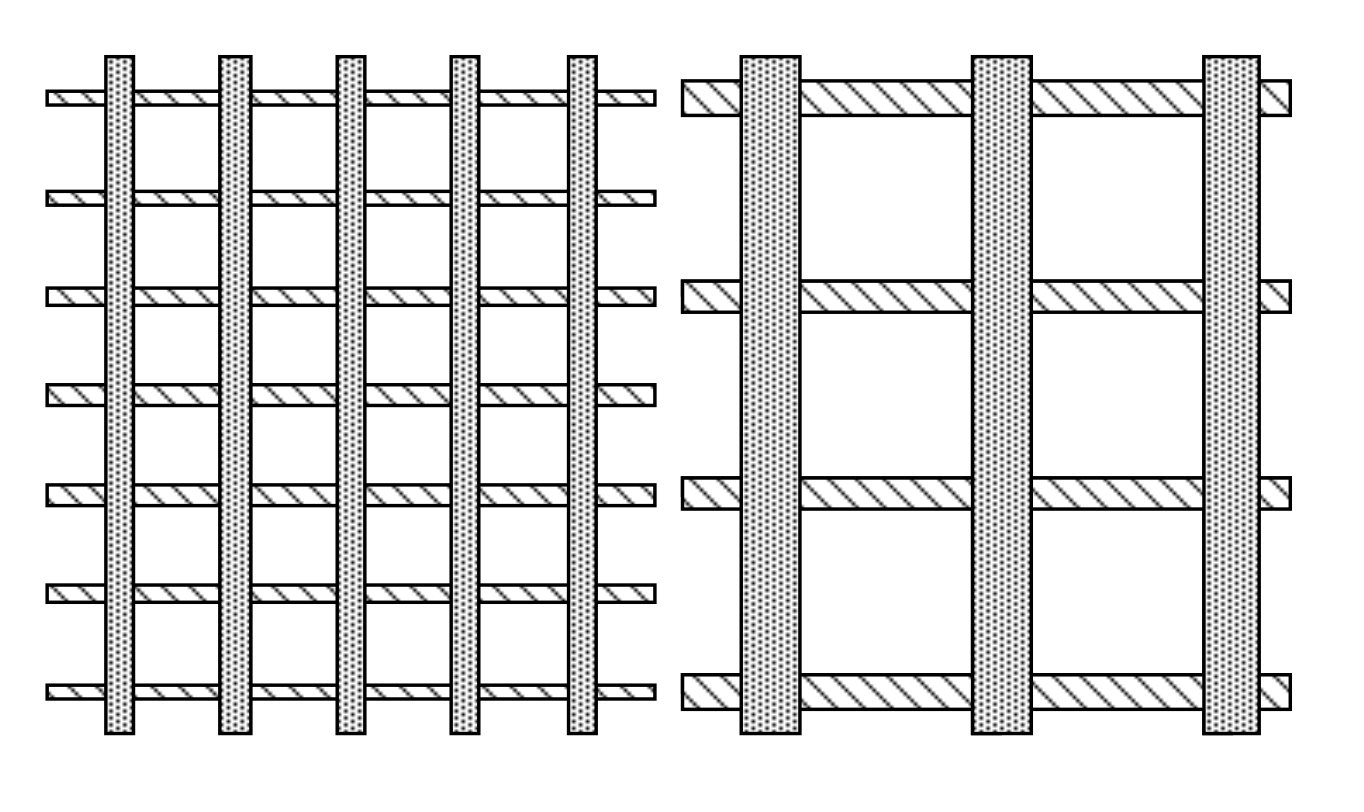
\includegraphics[height=6cm]{a8}
  \caption{供电网格的多种解析度}
  \label{fig:a7}
\end{figure}

一种有效的供电网格缩减方法是跳过所有其他导线,导致如图\ref{fig:a8}所示的情况。 然而,典型的供电网格可能是不规则的,即不同的边缘可能具有不同的长度和不同的间隔距离。 因此,网格缩减算法应该具有缩减任何一般网格的功能通用性。 此外,该算法应该保持原始的网格结构,使其可以被递归地应用,直到产生足够粗的网格。

网格缩减算法的主要目标是移除尽可能多的节点,同时保持通过插值估计被去除节点的电压的能力。 该算法将精细网格$\Omega^h$和要保留的节点列表作为输入,并输出具有较少数量节点的缩减网格$\Omega^{2h}$。 保留节点的列表应由用户感兴趣的特定节点组成,但我们的技术自动生成包含电压源所在的节点和角落节点的列表。


\begin{figure}[H] % use float package if you want it here
  \centering
  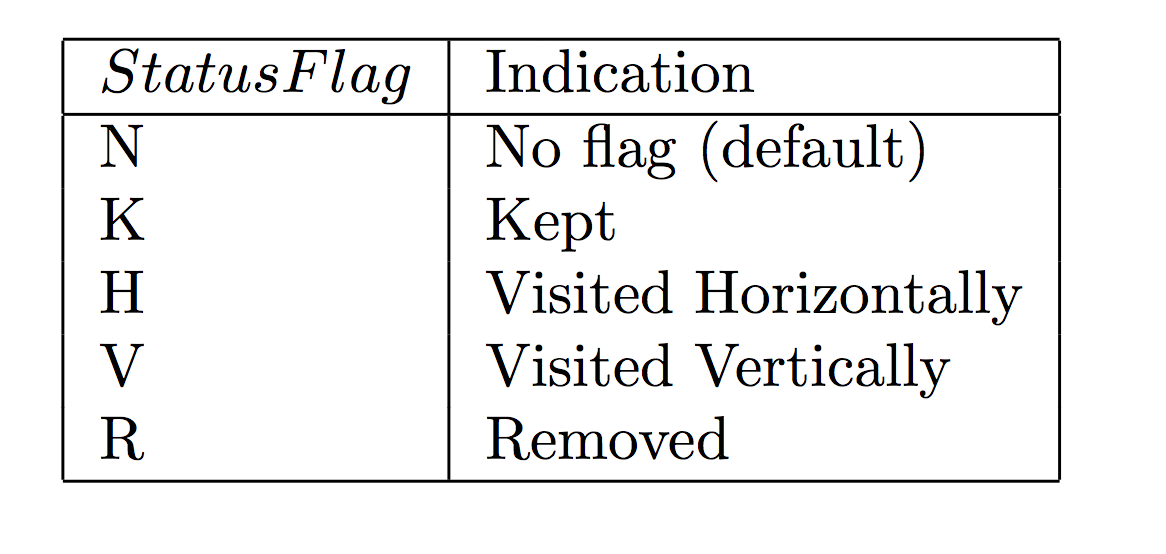
\includegraphics[height=4cm]{t1}
  \caption{状态标记的定义}
  \label{fig:t1}
\end{figure}

该算法利用表\ref{fig:t1}中说明的某些状态标志来确定节点是保留还是移除。 此外,这些标志指示如何从被保留的邻居插值获得已删除节点处的电压。 网格缩减算法重复使用所谓的节点更新操作,操作定义如下:从该节点开始沿着水平(垂直)方向,并用H(V)标记所有访问节点。 同时被水平和垂直访问的节点(标记为H和V)被标记为保留。 该算法由三个步骤组成,如下所述:
\begin{enumerate}
\item 第一步:对所有\emph{保留}节点进行\emph{更新操作};
\item 第二步:对于所有H(V)节点,标记它为R,表示移除;然后标记它沿着同一行(列)邻居为\emph{保留}并对其进行\emph{更新操作};如果一个节点没有被标记(N),那么标记它为移除(R),标记它的对角线上的邻居为\emph{保留}并进行\emph{更新操作};
\item 第三步:被保留的节点的电压值与它在粗网格上计算得来的值相同。一个H(V)节点(也就是被移除节点)的电压值由它的邻居(沿行或列方向)插值而来。标记为N的节点的电压值从它的被标记为\emph{保留}的对角邻居插值而得到。
\end{enumerate}
节点X的对角线邻居被定义为通过从水平方向首先前进一步,然后再垂直地走一步;或先垂直地然后水平地走一步而达到的那些节点。 例如,如果节点Y是节点X的上邻,则Y的左右邻居是X的对角邻居。

\begin{figure}[H] % use float package if you want it here
  \centering
  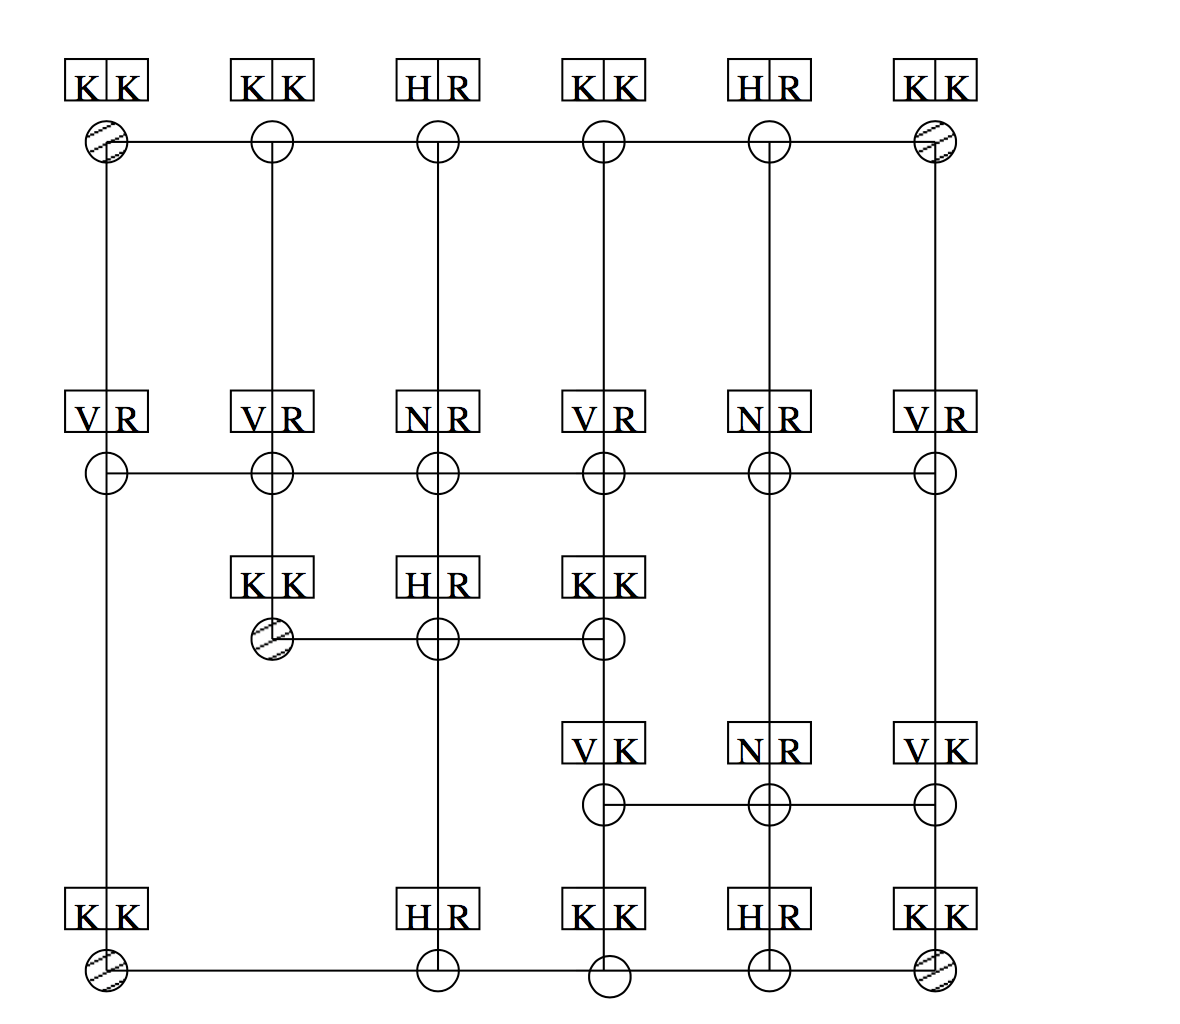
\includegraphics[height=9cm]{a9}
  \caption{对不规则网格的缩减示例}
  \label{fig:a9}
\end{figure}

该算法由图\ref{fig:a9}所示的不规则网格$\Omega^h$表示,其将被缩减而得到网格$\Omega^{2h}$。 在实施供电网格缩减算法时,网格节点从上到下、从左到右按顺序排列。 然而,值得注意的是,这不足够强大以处理任何的节点序列。

一开始,所有节点的默认状态为N,除了应保留的节点。 在这个例子中,被保留的节点将是网格的所有角落节点(图\ref{fig:a9}中的虚线节点)。 由两个字符组成的标签与网格的每个节点相关联。 左边字符表示第一次通过后节点的状态,右边字符表示第二次通过后节点的状态。

如图\ref{fig:a9}所示,在第一步完成之后,由至少一个保留节点组成的行或列的末端被标记为保留。 基于边缘是水平还是垂直的,边缘上的剩余节点用H或V标记。 注意到一些节点仍然具有N的状态标志,这表示在第一次通过期间这些节点未被访问。 然后在第二步完成之后,保留具有K标志的节点,而具有R标志的节点被去除,从而产生较粗的网格$\Omega^{2h}$。

\begin{figure}[H] % use float package if you want it here
  \centering
  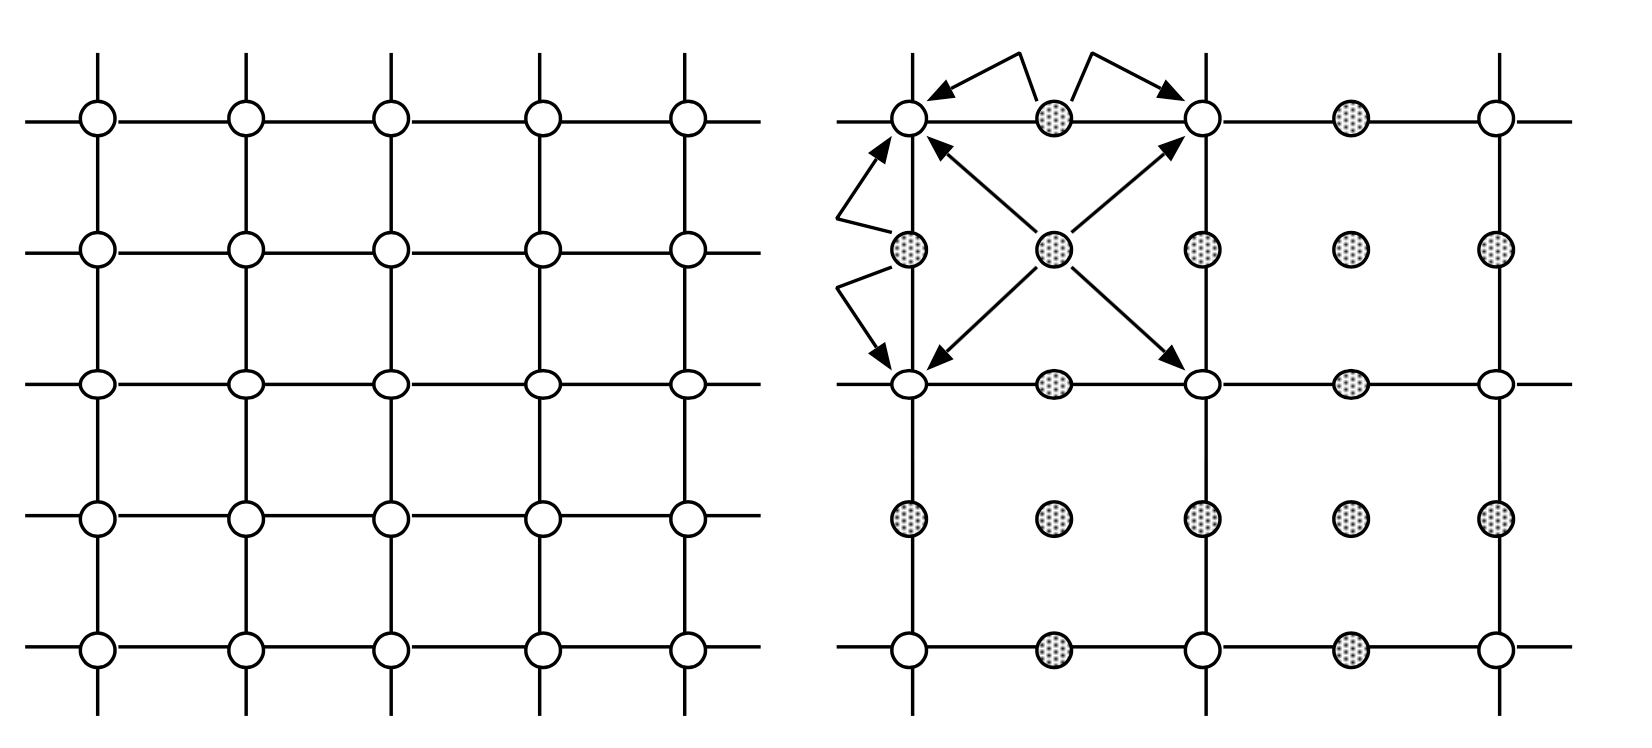
\includegraphics[height=7cm]{a10}
  \caption{基本的缩减操作}
  \label{fig:a10}
\end{figure}

最后,我们指出,如果原始网格是规则的,那么算法是最优的。 也就是说,它导致如图\ref{fig:a10}所示的例子中的节点数量达到最大的缩减。在这种情况下,每次网格缩减操作能产生一个线性方程组,其未知数数量减少约4倍,运行时的CPU时间减少约8倍。

\subsection{插值操作}

AMG的插值操作子应该使得:被去除的节点$i$的电压与和$i$强连接的那些被保留的节点的电压相关联。 通常来说,当$|a_{ij}|/\max_{l\neq i}|a_{il}|\geq \theta$,其中$0\leq \theta \leq 1$(在实践中$\theta$通常被选取为$0.25$)时,AMG会考虑两个节点$i$和$j$之间有强连接。 通过这种插值操作子的选择,粗网格校正可以有效地减少误差。

在我们的缩减算法中,状态标志指示删除的节点的哪些邻居将用于插值,而这取决于它们被保留并且与被去除的节点$m$强连接。 对于插值权重,可以通过考虑节点间的电导值来获得。 因此,如果用节点$A$和$B$处的电压插值得到被去除节点$m$处的电压,则他们的(线性)插值函数INT()定义为:
\begin{align}
V(m)=\text{INT}(V(A),V(B))=a_0V(A)+a_1V(b)
\end{align}
其中$a_0=\frac{g_{mA}}{g_{mA}+g_{mB}}$,并且$a_1=\frac{g_{mB}}{g_{mA}+g_{mB}}$。在这里,$g_{mA}$表示节点$m$与节点$A$之间的电导,$g_{mB}$表示节点$m$与节点$B$之间的电导。注意到我们选取插值权重的方法来源于代数
多重网格中的类似方法。为了说明,考虑一个被取出节点$m$,它的电压会从保留节点$A$与$B$中插值而得来。代数多重网格方法使用下面的插值方法:
\begin{align}
V(m)=\frac{|a_{mA}|}{a_{mm}}V(A)+\frac{|a_{mB}|}{a_{mm}}V(B)
\end{align}
其中$a_{mA}$是矩阵$A$中与$m$与$A$关联的元素,$a_{mB}$是矩阵$A$中与$m$与$B$关联的元素。至于$a_{mm}$,一种代数多重网格中的方法是把它定义为矩阵中$m$对应的对角元素。另一种多重网格中的方法是定义为:$a_{mm}=|a_{mA}|+|a_{mB}|$。在供电网格
方法中,$|a_{mA}|=g_{mA}$,且$|a_{mB}|=g_{mB}$,这说明我们的插值方法来源于代数多重网格方法。

\begin{figure}[H] % use float package if you want it here
  \centering
  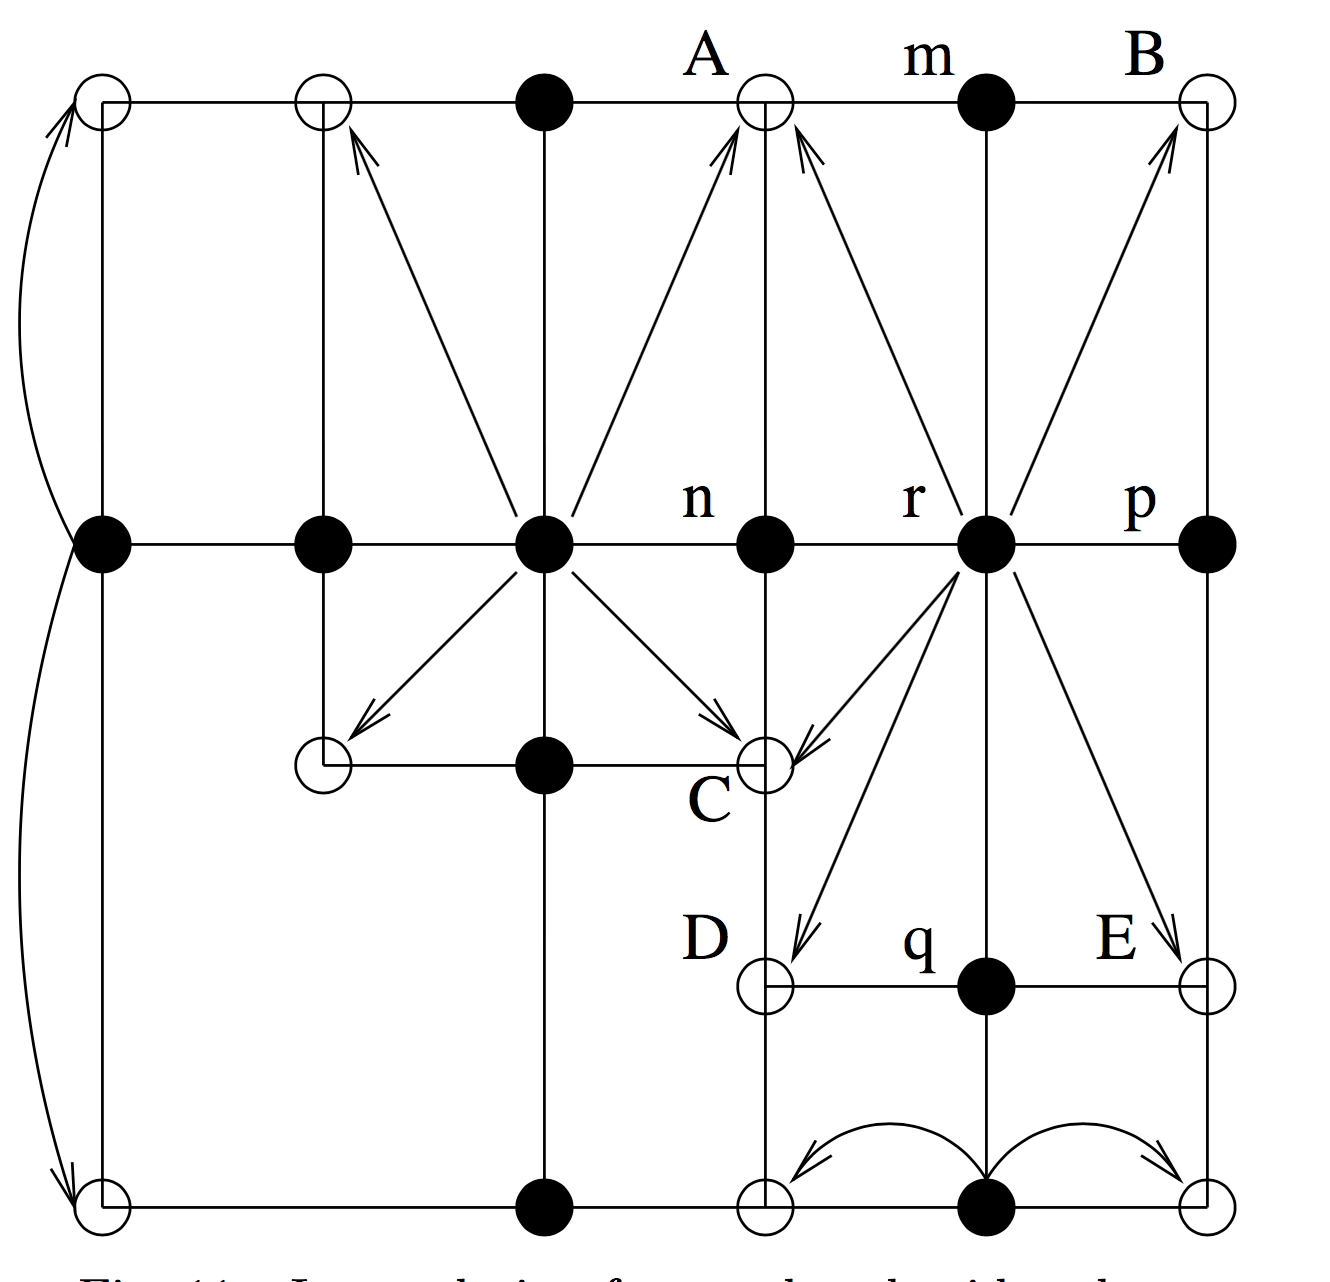
\includegraphics[height=7cm]{a11}
  \caption{在缩减网格中进行插值操作}
  \label{fig:a11}
\end{figure}

然而,这还不是全部。回想一下,我们的供电网格缩减算法与代数多重网格缩减方法不同;它实际上是基于标准多重网格算法的缩减算法,它只使用了几何信息,并删除尽可能多的节点。因此,有可能遇到被移除节点$i$的与其强连接的所有节点也被删除的情况。为了说明这一点,考虑图\ref{fig:a11},其中实心节点指示被去除的节点,空心节点指示保留的节点。在这个例子中,我们假设每个水平或垂直连接都代表一个强连接,但由两个或更多个连接分开的节点间并没有强连接。这种情况是供电网格的典型情况。因此,r与m强连接,m与B强连接,但r和B不连接。这种类似于B的节点,与r之间没有强连接但是通过两个强连接能与r有关系的节点,我们称它们与r\emph{二度强连接}。我们的网格缩减将删除节点r,以及强烈连接到它的所有节点,m,n,p和q。然而,可以发现,我们的算法保证,如果删除节点i,则保留与i强连接的一些节点,或者保留与i\emph{二度强连接}的一些节点。因此,在我们的插值技术中,如果一个节点的所有强连接的邻居与它一起被去除,我们使用它的\emph{二度强连接}的保留的邻居节点进行插值。这在图\ref{fig:a11}中能清楚地看出。,其中节点r处的电压从\emph{二度强连接}到r的那些节点插值而得到;具体来说,是节点A,B,C,D和E。注意,这种方法保持了有效网格减少的优点,同时满足了良好的插值操作子的要求。
